\addtocontents{toc}{\protect\vfill\newpage}  %ToC would split algorithms chapter otherwise
\chapter{Algorithms} \label{chap:algorithms}

The iterations and data accessors described in the previous Chapters allow for a plethora of algorithms.
Most of them make use of basic functionalities such as the inner product of vectors, or the volume of a $n$-cell.
{\ViennaGrid} ships with a number of such basic tools, which are listed in Tab.~\ref{tab:algorithms} and discussed in the following.

The individual algorithms are located in the \lstinline|viennagrid/algorithm/| folder.
A tutorial covering the algorithms explained in this chapter can be found in \lstinline|examples/tutorial/algorithms.cpp|.


\TIP{Make sure to include the respective header-file when using one of the algorithms explained below!}

\begin{table}
 \begin{tabular}{|l|l|l|}
  \hline
   Algorithm & Filename   & Interface Function\\
   \hline
   Cross Product & \texttt{cross\_prod.hpp} & \lstinline|cross_prod(a, b)| \\
   Inner Product & \texttt{inner\_prod.hpp} & \lstinline|inner_prod(a, b)|\\
   Vector Norms & \texttt{norm.hpp} & \lstinline|norm(a, tag)| \\
   Induced Volume & \texttt{spanned\_volume.hpp} & \lstinline|spanned_volume(a, b, ...)| \\
   \hline
   Centroid computation & \texttt{centroid.hpp} & \lstinline|centroid(element)| \\
   Circumcenter comp. & \texttt{circumcenter.hpp} & \lstinline|circumcenter(element)| \\
   Surface computation & \texttt{surface.hpp} & \lstinline|surface(element)| \\
   Volume computation & \texttt{volume.hpp} & \lstinline|volume(element)| \\
   \hline
   Boundary detection & \texttt{boundary.hpp} & \lstinline|is_boundary(domseg, element)|\\
   Interface detection & \texttt{interface.hpp} & \lstinline|is_interface(seg1, seg2, element)|\\
   Simplex refinement & \texttt{refine.hpp} & \lstinline|refine(tag, domain)| \\
   Surface computation & \texttt{surface.hpp} & \lstinline|surface(domseg)| \\
   Volume computation & \texttt{volume.hpp} & \lstinline|volume(domseg)| \\
   Voronoi grid & \texttt{voronoi.hpp} & \lstinline|apply_voronoi(domseg, ...)| \\
   \hline
 \end{tabular}
 \caption{List of algorithms available in \texttt{viennagrid/algorithm/} grouped by the objects they are acting on. 
    \lstinline|a| and \lstinline|b| denote vectors, \lstinline|element| refers to an element,
    \lstinline|domain| to a domain, \lstinline|seg1| and \lstinline|seg2| to segments, and \lstinline|domseg| to either a domain or a segment.}
 \label{tab:algorithms}
\end{table}


\section{Point/Vector-Based}
This section details algorithms in {\ViennaGrid} requiring geometric information only.
The point type in {\ViennaGrid} should be seen in this context mostly as a vector type rather than a representation of a geometric location, reflecting the duality of points and vectors in the Euclidian space.

  \subsection{Cross Products}
 The cross-product of two vectors (i.e.~{\ViennaGrid} points) $p0$ and $p1$ is defined for the three-dimensional space and computed with {\ViennaGrid} as
 \begin{lstlisting}
  viennagrid::cross_prod(p1, p2)
 \end{lstlisting}
 The following code calculates and prints the cross-product of the vectors $(1,0,0)^\mathrm{T}$ and $(0,1,0)^\mathrm{T}$:
 \begin{lstlisting}
  PointType p0(1, 0, 0);
  PointType p1(0, 1, 0);
  std::cout << viennagrid::cross_prod(p1, p2) << std::endl; //0 0 1
 \end{lstlisting}
 If the two vectors are given in different coordinate systems, the result vector will have the same coordinate system as the first argument.
  

  \subsection{Inner Products}
 Unlike cross products, inner products (aka.~dot products) are well defined for arbitrary dimensions. In {\ViennaGridversion} an inner product of the form
\begin{align}
 (\vector x, \vector y) = \sum_{i=0}^{N-1} x_i y_i
\end{align}
is available with the function \lstinline|inner_prod()|. The following code calculates and prints the inner product of the vectors $(1,0,0)^\mathrm{T}$ and $(0,1,0)^\mathrm{T}$:
 \begin{lstlisting}
  PointType p0(1, 0, 0);
  PointType p1(0, 1, 0);
  std::cout << viennagrid::inner_prod(p1, p2) << std::endl;  //0
 \end{lstlisting}
 If the two vectors are given in different coordinate systems, the result vector will have the same coordinate system as the first argument.
 
  \subsection{Vector Norms}
 Currently, $p$-norms of the form
  \begin{align}
   \Vert x \Vert_p = \sqrt[p]{\sum_{i=0}^{N-1} x_i^p}
  \end{align}
 are implemented in the $N$-dimensional Euclidian space for $p=1$, $p=2$ and $p=\infty$. The three norms for the vector $(1,2,3)^\mathrm{T}$ are computed and printed using the lines
 \begin{lstlisting}
  PointType p(1, 2, 3);
  std::cout << viennagrid::norm_1(p)   << std::endl; //6
  std::cout << viennagrid::norm_2(p)   << std::endl; //3.74
  std::cout << viennagrid::norm_inf(p) << std::endl; //3
 \end{lstlisting}
which are equivalent to
 \begin{lstlisting}
  PointType p(1, 2, 3);
  std::cout << viennagrid::norm(p, viennagrid::one_tag()) << std::endl;
  std::cout << viennagrid::norm(p, viennagrid::two_tag()) << std::endl;
  std::cout << viennagrid::norm(p, viennagrid::inf_tag()) << std::endl;
 \end{lstlisting}
 

  \subsection{Volume of a Spanned Simplex}
  It is often handy to compute the $n$-dimensional volume of a $n$-simplex embedded in a possibly higher-dimensional geometric space by providing the locations of the vertices only.
  This is provided by \lstinline|spanned_volume()|, which is, however, currently limited to $n \in \{1, 2, 3\}$.
  As an example, the two-dimensional volume a triangle with corners at $(1, 0, 0)$, $(2, 1, 1)$ and $(1, 1, 2)$ is computed and printed by
  \begin{lstlisting}
   PointType p0(1, 0, 0);
   PointType p1(2, 1, 1);
   PointType p2(1, 1, 2);
   std::cout << viennagrid::spanned_volume(p0, p1, p2) << std::endl;
  \end{lstlisting}



\section{Element-Based}
In this section, algorithms defined for geometric objects with additional structure are discussed. Additional algorithms are likely to be introduced in future releases.
 
  \subsection{Centroid}
  The centroid of an element object \lstinline|element| in Cartesian coordinates is obtained as
  \begin{lstlisting}
   PointType p = viennagrid::centroid(cell_n);
  \end{lstlisting}
  and works for arbitrary topological and geometrical dimensions.

  \subsection{Circumcenter}
  The circumcenter of a simplex \lstinline|element| is obtained in Cartesian coordinates as
  \begin{lstlisting}
   PointType p = viennagrid::circumcenter(element);
  \end{lstlisting}
  The computation is restricted to simplices of topologic dimension $n \leq 3$. For reasons of uniformity, also hypercubes can be passed, for which the circumcenter of an embedded simplex is computed. This leads to valid results and makes sense only for certain regular hypercubes.
  Thus, the user has to ensure that the hypercube actually has a circum-sphere. This is e.g.~the case for structured tensor-grids.

 \NOTE{There is no warning or error issued if a hypercube passed to \lstinline|circumcenter()| does not have a circumcenter.}

  \subsection{Surface}
  The surface of an element \lstinline|element| is defined as the sum of the volumes of its facet elements. Therefore, in order to make the calling code
  \begin{lstlisting}
   NumericType surf = viennagrid::surface(element);
  \end{lstlisting}
%   valid, the storage of $n-1$-cells at the boundary of $n$-cells must not be disabled, cf.~Section \ref{subsec:boundary-ncells-storage}.
  Currently, \lstinline|surface()| is restricted to element with topologic dimension $n \leq 4$.

%   \NOTE{In order to use \lstinline|surface()| for a $n$-cell $T_n$, make sure that boundary $n-1$-cells are not disabled, cf.~Section \ref{subsec:boundary-ncells-storage}.}

  \subsection{Volume}
  The $n$-dimensional volume of an element \lstinline|element| is returned by
  \begin{lstlisting}
   NumericType vol = viennagrid::volume(element);
  \end{lstlisting}
  and currently restricted to elements with topologic dimension $n \leq 3$. No restrictions with respect to the storage of boundary elements apply.


\section{Domain/Segment-Based}
Algorithms acting on a collection of cells are now considered. These collections are given in {\ViennaGrid} either as the whole domain, or as segments.

 \subsection{Boundary}
 Whether or not an element object \lstinline|element| is located on the boundary depends on the collection of elements considered.
 For example, consider the edge/facet $[1,4]$ in the triangular sample mesh in Fig.~\ref{fig:sampledomain}, which we will refer to as \lstinline|f|.
 It is in the interior of the whole \lstinline|domain|, while it is also at the boundary of the two segments \lstinline|seg0| and \lstinline|seg1|.
 A sample code snippet reflecting this is given by
 \begin{lstlisting}
  std::cout << viennagrid::is_boundary(domain, f) << std::endl; //false;
  std::cout << viennagrid::is_boundary(seg0, f)   << std::endl; //true;
  std::cout << viennagrid::is_boundary(seg1, f)   << std::endl; //true;
 \end{lstlisting}
 Note that \lstinline|is_boundary()| induces some additional setup costs at the first time the function is called. However, subsequent calls are accelerated and will usually compensate for the setup costs.

%  \NOTE{\lstinline|is_boundary| requires that facets are stored within cells. Therefore, make sure not to disable the handling of facets, cf.~Section \ref{subsec:boundary-ncells-storage}. }
 

 \subsection{Interface}
  Similar to the detection of boundary facets, elements on the interface between two segments are frequently of particular interest. 
  An element \lstinline|element| can be checked for being on the interface of two segments \lstinline|seg0| and \lstinline|seg1| using
 \begin{lstlisting}
  std::cout << viennagrid::is_interface(seg0, seg1, element) << std::endl;
 \end{lstlisting}
 Note that \lstinline|is_interface()| induces some setup costs the first time it is called for a pair of segments.

%  \NOTE{\lstinline|is_interface()| requires that facets are stored within cells. Therefore, make sure not to disable the handling of facets, cf.~Section \ref{subsec:boundary-ncells-storage}. }


 \subsection{Refinement}
 {\ViennaGridversion} allows a uniform and a local refinement of simplicial domains. The refinement of hypercuboidal domains is scheduled for future releases.
It has to be noted that the resulting refined mesh is written to a new domain, thus there are no multigrid/multilevel capabilities provided yet.

 To refine a \lstinline|domain| uniformly, the line
 \begin{lstlisting}
 DomainType refined_domain;
 viennagrid::refine_uniformly(domain, refined_domain);
 \end{lstlisting}
 is sufficient.
 
 Refinement is also supported for domains with segmentations. Segment information is preserved upon refinement.
 \begin{lstlisting}
 DomainType refined_domain;
 SegmentationType refined_segmentation;
 viennagrid::refine_uniformly(domain,         segmentation,
                              refined_domain, refined_segmentation);
 \end{lstlisting}

 The local refinement of a mesh requires that the respective cells or edges for refinement are tagged. This refinement information is applied to the domain using accessors or fields, cf.~Chapter \ref{chap:data}.
 First of all a tag container and an accessor has to be created:
 \begin{lstlisting}
 std::vector<bool> cell_refinement_container;
 viennagrid::result_of::accessor<std::vector<bool>, CellType>::type cell_refinement_accessor(cell_refinement_container);
 \end{lstlisting}
 
 
 To tag a cell \lstinline|c| for refinement, the line
 \begin{lstlisting}
 cell_refinement_accessor(c) = true;
 \end{lstlisting}
 is sufficient. In a similar way one proceeds for other cells or edges in the domain. The refinement process is then triggered by
 \begin{lstlisting}
 DomainType refined_domain;
 viennagrid::cell_refine(domain, refined_domain, cell_refinement_accessor);
 \end{lstlisting}
 
 \pagebreak
 
 or, for segmentations
 \begin{lstlisting}
 DomainType refined_domain;
 SegmentationType refined_segmentation;
 viennagrid::cell_refine(domain,         segmentation,
                         refined_domain, refined_segmentation,
                         cell_refinement_accessor);
 \end{lstlisting}
%  Again, no expensive temporary domain is created for the refinement process thanks to the use of a proxy object.

%  \NOTE{\lstinline|refine()| requires edges to be stored in the domain. Make sure not to disable the handling of edges, cf.~Section \ref{subsec:boundary-ncells-storage}. }

 \subsection{Surface}
 The surface of a domain or segment \lstinline|domseg| is given by the sum of the volumes of the boundary facets and returned by the convenience overload
  \begin{lstlisting}
   NumericType surf = viennagrid::surface(domseg);
  \end{lstlisting}
  Note that facets interfacing cells outside the segment are also considered as boundary facets of the segment.

%   \NOTE{In order to use \lstinline|surface()| for a domain or a segment, make sure that boundary $n-1$-cells are not disabled, cf.~Section \ref{subsec:boundary-ncells-storage}.}

  \subsection{Volume}
  The volume of a domain or segment \lstinline|domseg| is returned by
  \begin{lstlisting}
   NumericType vol = viennagrid::volume(domseg);
  \end{lstlisting}
  and currently restricted to maximum topological dimension $n \leq 3$.



\begin{figure}[tb]
\centering
 \psfrag{i}{$i$}
 \psfrag{j}{$j$}
 \psfrag{Aij}{$A_{[i,j]}$}
 \psfrag{Vij}{$V_{[i,j]}$}
 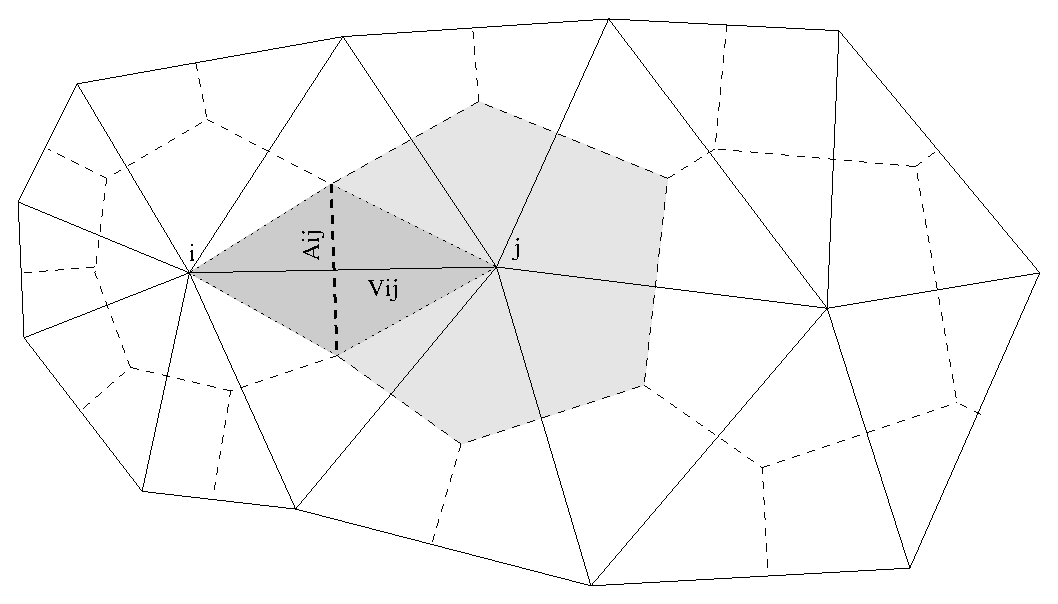
\includegraphics[width=0.9\textwidth]{figures/voronoi.eps}
 \caption{Schematic of a Delaunay mesh with its dual Voronoi diagram, where the box containing vertex $j$ is highlighted.
    The function \lstinline|voronoi()| computes and stores the Voronoi volume $V_{[i,j]}$ and the interface area $A_{[i,j]}$ associated with each edge $[i,j]$.
    The total box volume associated with each vertex is also stored on the vertex.}
 \label{fig:voronoi}
\end{figure}

 \subsection{Voronoi Information}
 A Voronoi diagram of a Delaunay tessellation (or triangulation) is a decomposition of the domain into certain boxes containing one vertex each.
 The boxes have the property that all points inside the box are closer to the vertex within the box than to any other vertex in the domain. 
 By simple geometric arguments one finds that the corners of Voronoi boxes are given by the circumcenters of the triangles.

 The function \lstinline|apply_voronoi()| computes the volumes and interfaces associated with a Voronoi diagram. The following values are stored on the domain (cf.~Fig.~\ref{fig:voronoi})
 \begin{itemize}
  \item The volume $V_{[i,j]}$ of the polyhedron centered around the edge $[i,j]$ with edges given by the connections of the vertices $i$ and $j$ with the circumcenters of the coboundary cells of the edge is stored on the edge $[i,j]$.
  \item The interface area $A_{[i,j]}$ of the boxes for the vertices $i$ and $j$ on the edge $[i,j]$.
  \item The box volume $V_i$ of the box containing vertex $i$ for each vertex $i$.
 \end{itemize}
 Using the lines
 \begin{lstlisting}
  using namespace viennagrid;
  typedef result_of::voronoi_cell_contribution<ConstCellHandleType>::type ContributionType;
 
  std::vector<double> interface_areas;
  std::vector<ContributionType> interface_contributions;
  
  result_of::accessor< std::vector<double>, EdgeType >::type interface_areas_accessor(interface_areas);
  result_of::accessor< std::vector<ContributionType>, EdgeType >::type interfaces_contribution_accessor(interface_contributions);
  
  std::vector<double> vertex_box_volumes;
  std::vector<ContributionType> vertex_box_volume_contributions;
  
  result_of::accessor< std::vector<double>, VertexType >::type vertex_box_volumes_accessor(vertex_box_volumes);
  result_of::accessor< std::vector<ContributionType>, VertexType >::type vertex_box_volume_contributions_accessor(vertex_box_volume_contributions);
  
  std::vector<double> edge_box_volumes;
  std::vector<ContributionType> edge_box_volume_contributions;
  
  result_of::accessor< std::vector<double>, EdgeType >::type edge_box_volumes_accessor(edge_box_volumes);
  result_of::accessor< std::vector<ContributionType>, EdgeType >::type edge_box_volume_contributions_accessor(edge_box_volume_contributions);
  
  apply_voronoi<CellType>(
        domain,
        interface_areas_accessor, interfaces_contribution_accessor,
        vertex_box_volumes_accessor, vertex_box_volume_contributions_accessor,
        edge_box_volumes_accessor, edge_box_volume_contributions_accessor)
  );
 \end{lstlisting}
 
 The voronoi values are stored in the corresponding accessors/containers.
